
%(BEGIN_QUESTION)
% Copyright 2007, Tony R. Kuphaldt, released under the Creative Commons Attribution License (v 1.0)
% This means you may do almost anything with this work of mine, so long as you give me proper credit

A hydraulic system consisting of a hand-actuated {\it spool valve} and a double-acting {\it cylinder} may be thought of as a sort of control system.  Input (motion to the spool valve) results in a certain output (cylinder motion):

$$\includegraphics[width=15.5cm]{i02420x01.eps}$$

Identify what the arrows mean inside the spool valve symbol, and then explain whether you think the action of this ``control system'' is more like {\it proportional} or more like {\it integral}.

\underbar{file i02420}
%(END_QUESTION)





%(BEGIN_ANSWER)

The arrows represent hydraulic fluid direction.  Each of the three ``boxes'' in the spool valve symbol represents three different positions of the valve spool.

%(END_ANSWER)





%(BEGIN_NOTES)

The ``action'' of this system is {\it integral}, not proportional, if you consider the spool valve actuating lever to be the input (representing PV $-$ SP in a controller) and the cylinder position to be the output.  The lever's position controls the cylinder's {\it speed} rather than its {\it position}.

%INDEX% Control, integral: hydraulic spool valve and double-acting cylinder
%INDEX% Mechanics, fluid power systems: reversing (double-acting) cylinder control

%(END_NOTES)


